\pdfminorversion=4
\documentclass[aspectratio=169]{beamer}

\mode<presentation>
{
  \usetheme{default}
  \usecolortheme{default}
  \usefonttheme{default}
  \setbeamertemplate{navigation symbols}{}
  \setbeamertemplate{caption}[numbered]
  \setbeamertemplate{footline}[frame number]  % or "page number"
  \setbeamercolor{frametitle}{fg=white}
  \setbeamercolor{footline}{fg=black}
} 

\usepackage[english]{babel}
\usepackage[utf8x]{inputenc}
\usepackage{tikz}
\usepackage{courier}
\usepackage{array}
\usepackage{bold-extra}
\usepackage{minted}
\usepackage[thicklines]{cancel}
\usepackage{fancyvrb}

\xdefinecolor{dianablue}{rgb}{0.18,0.24,0.31}
\xdefinecolor{darkblue}{rgb}{0.1,0.1,0.7}
\xdefinecolor{darkgreen}{rgb}{0,0.5,0}
\xdefinecolor{darkgrey}{rgb}{0.35,0.35,0.35}
\xdefinecolor{darkorange}{rgb}{0.8,0.5,0}
\xdefinecolor{darkred}{rgb}{0.7,0,0}
\definecolor{darkgreen}{rgb}{0,0.6,0}
\definecolor{mauve}{rgb}{0.58,0,0.82}

\title[2020-10-01-lhcb-computing]{\only<1>{Future of}\only<2>{\xcancel{Future of} Trends in} User Analysis}
\author{Jim Pivarski}
\institute{Princeton University -- IRIS-HEP}
\date{October 1, 2020}

\usetikzlibrary{shapes.callouts}

\begin{document}

\logo{\pgfputat{\pgfxy(0.11, 7.4)}{\pgfbox[right,base]{\tikz{\filldraw[fill=dianablue, draw=none] (0 cm, 0 cm) rectangle (50 cm, 1 cm);}\mbox{\hspace{-8 cm}
\includegraphics[height=1 cm]{princeton-logo-long.png}\hspace{0.1 cm}\raisebox{0.1 cm}{
\includegraphics[height=0.8 cm]{iris-hep-logo-long.png}}\hspace{0.1 cm}}}}}

\begin{frame}
  \titlepage
\end{frame}

\logo{\pgfputat{\pgfxy(0.11, 7.4)}{\pgfbox[right,base]{\tikz{\filldraw[fill=dianablue, draw=none] (0 cm, 0 cm) rectangle (50 cm, 1 cm);}\mbox{\hspace{-8 cm}
\includegraphics[height=1 cm]{princeton-logo.png}\hspace{0.1 cm}\raisebox{0.1 cm}{
\includegraphics[height=0.8 cm]{iris-hep-logo.png}}\hspace{0.1 cm}}}}}

% Uncomment these lines for an automatically generated outline.
%\begin{frame}{Outline}
%  \tableofcontents
%\end{frame}

% START START START START START START START START START START START START START

\begin{frame}{Define: ``user analysis''}
\large
\vspace{0.5 cm}

I'm aware that LHCb is moving important physics decisions earlier in the pipeline, but I think it's still meaningful to talk about ``user analysis'' as the last step.

\begin{center}
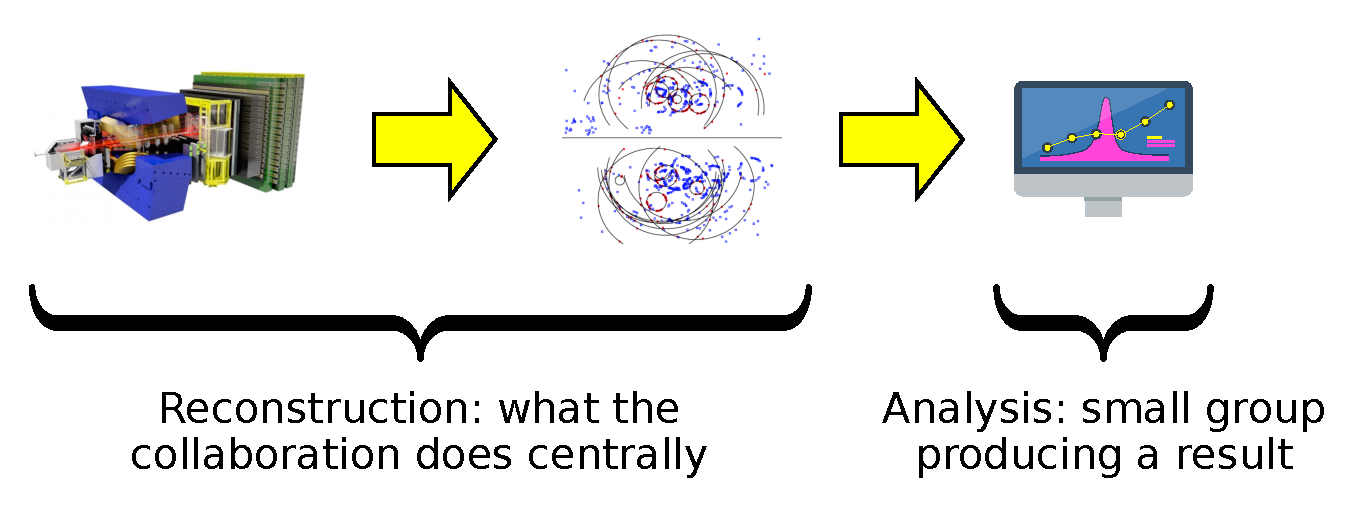
\includegraphics[width=0.9\linewidth]{img/analysis-pipeline.pdf}
\end{center}
\end{frame}

\begin{frame}{\mbox{ }}
\vspace{0.5 cm}

\begin{center}
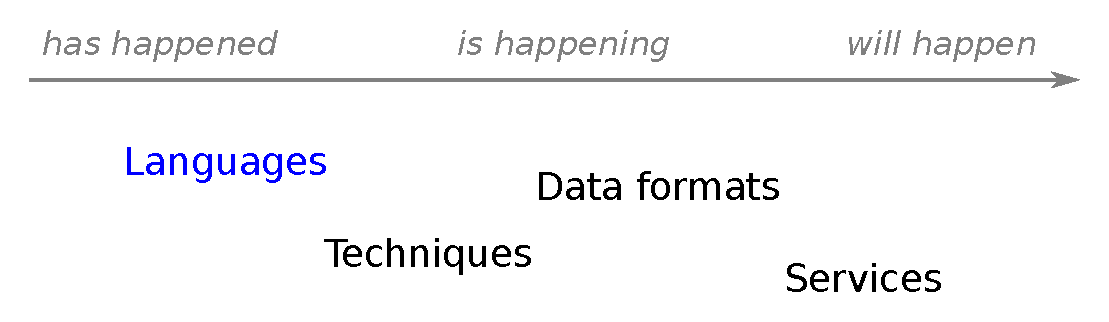
\includegraphics[width=0.9\linewidth]{img/topics-1.pdf}
\end{center}
\end{frame}

\begin{frame}{Python: the revolution has already happened}
\large
\vspace{0.35 cm}

Plot \#1: pip-install statistics in the past three years

\normalsize
\textcolor{gray}{iminuit, root-numpy, and rootpy predate the rise, and therefore set the scale.}

\begin{center}
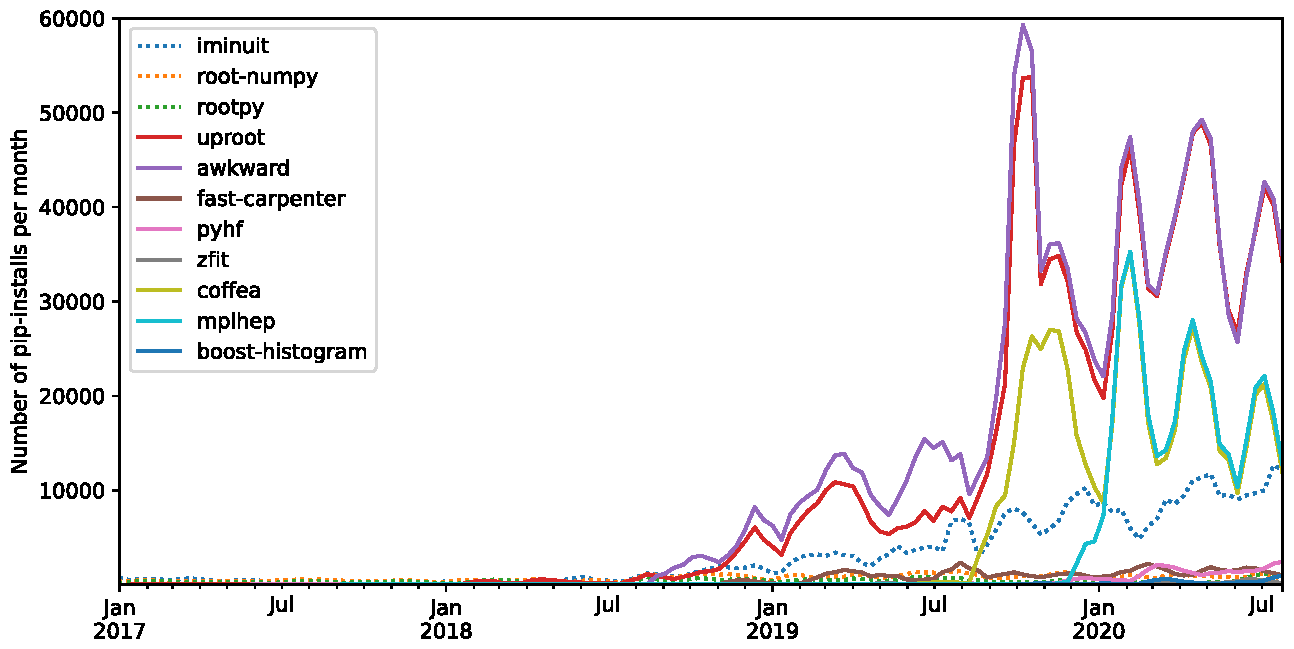
\includegraphics[width=0.85\linewidth]{img/piplinear-iminuit-rootnumpy-rootpy-uproot-awkward-fastcarpenter-pyhf-zfit-coffea-mplhep-boosthistogram.pdf}
\end{center}
\end{frame}

\begin{frame}{Python: the revolution has already happened}
\large
\vspace{0.35 cm}

Plot \#2: Language of non-fork GitHub repos by users who forked CMSSW

\normalsize
\vspace{\baselineskip}

\begin{center}
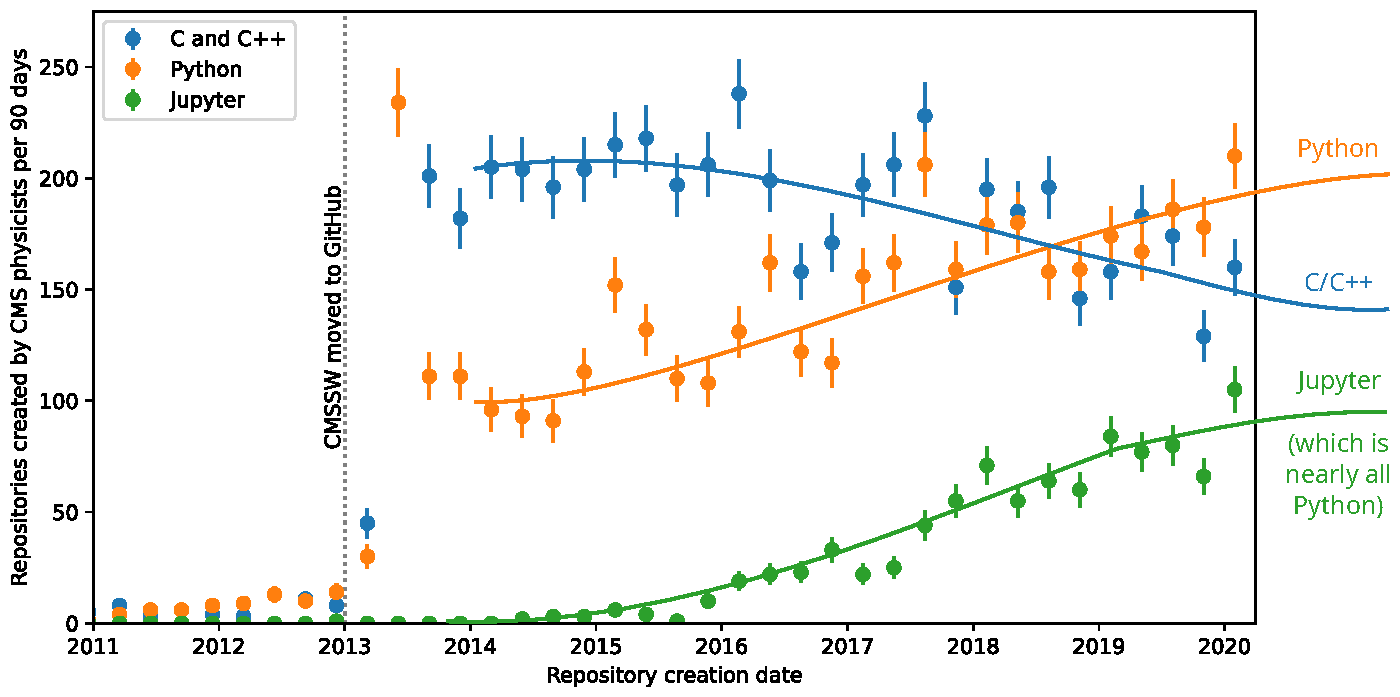
\includegraphics[width=0.85\linewidth]{img/01-github-cmssw-language.pdf}
\end{center}
\end{frame}

\begin{frame}{Python: the revolution has already happened}
\large
\vspace{0.35 cm}

Plot \#3: Search for substrings in those repos: what are those users typing?

\normalsize
\textcolor{gray}{We assume ``tfile'' correlates to ROOT; just ``root'' (case insensitive) is too generic.}

\begin{center}
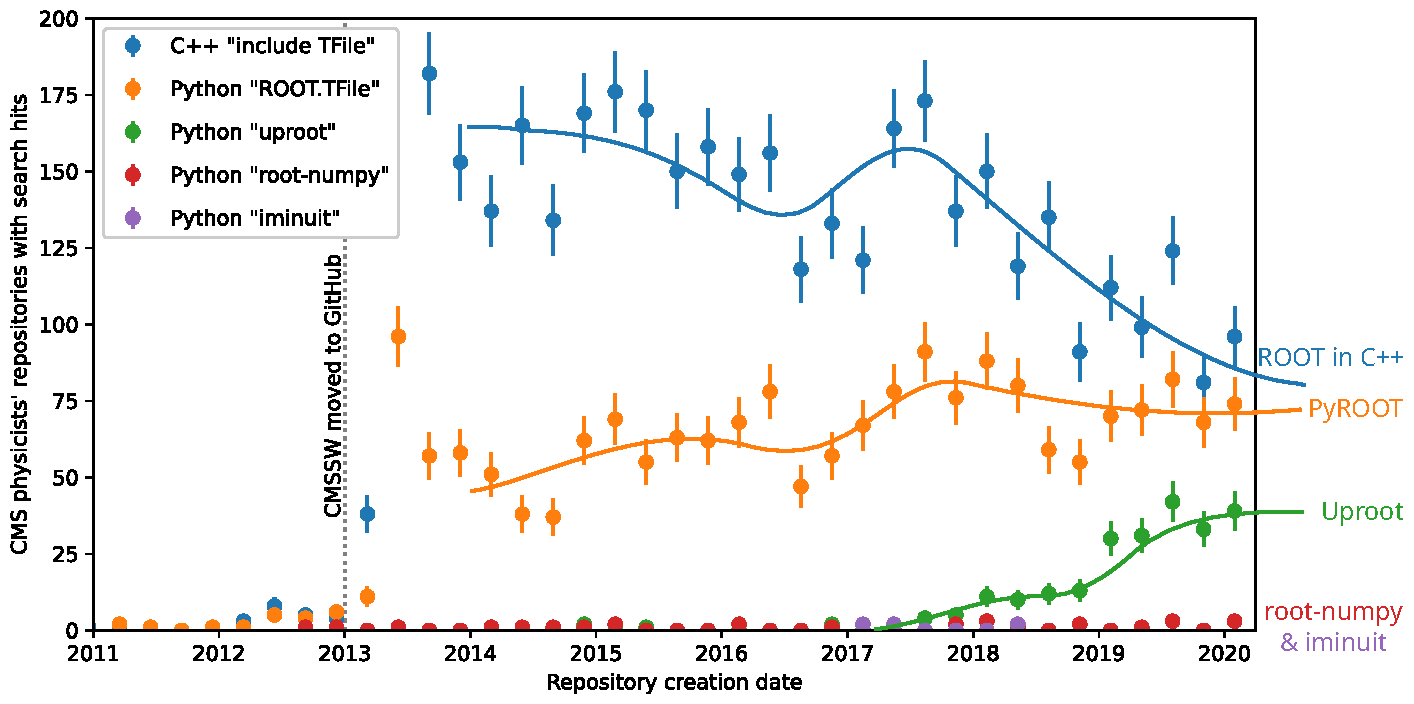
\includegraphics[width=0.85\linewidth]{img/03-github-root-python.pdf}
\end{center}
\end{frame}

\begin{frame}{Python: the revolution has already happened}
\large
\vspace{0.35 cm}

Plot \#3: What about machine learning?

\normalsize
\textcolor{gray}{{\bf Surprise:} Scikit-Learn! {\bf Not a surprise:} TMVA is the only significant C++ library.}

\begin{center}
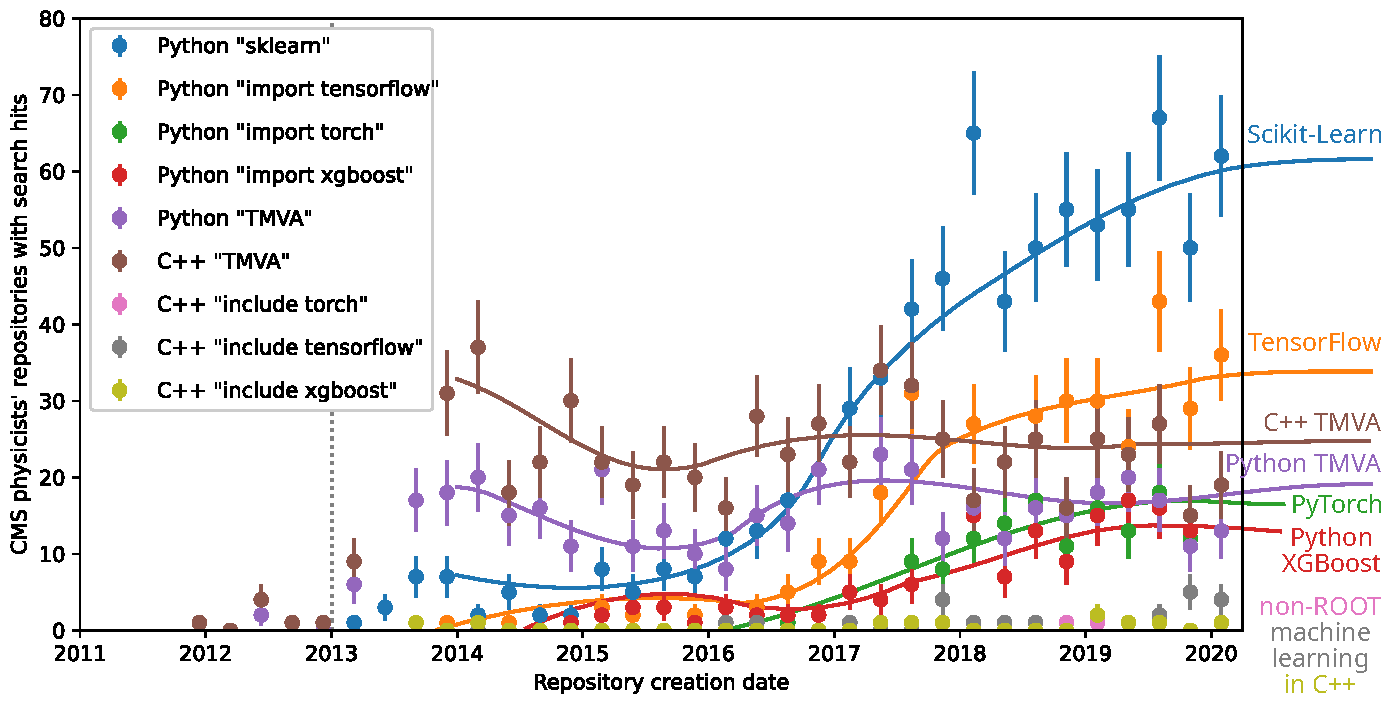
\includegraphics[width=0.85\linewidth]{img/04-github-machine-learning.pdf}
\end{center}
\end{frame}

\begin{frame}{Python: the revolution has already happened}
\large
\vspace{0.35 cm}

Plot \#4: Was Python adoption driven by Uproot or machine learning?

\normalsize
\textcolor{gray}{Twice as much basic analysis (NumPy/Matplotlib) than ML; trend predates Uproot.}

\begin{center}
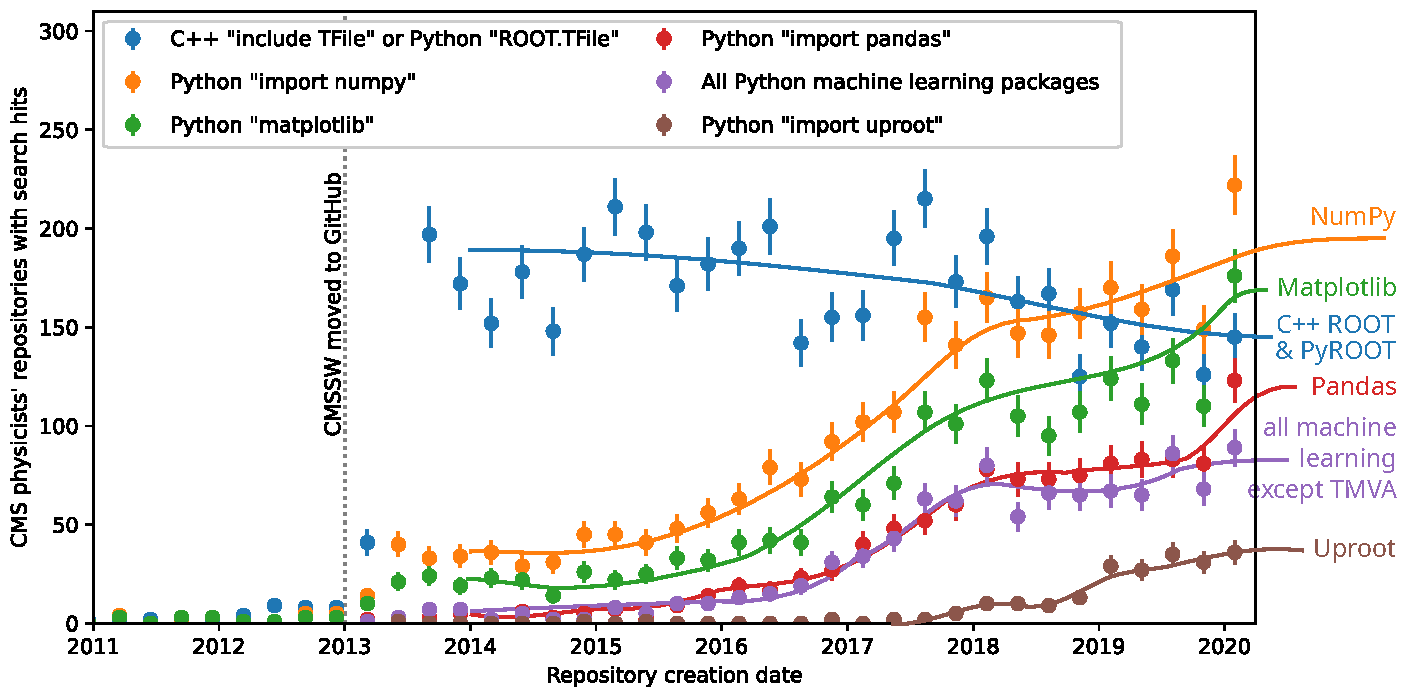
\includegraphics[width=0.85\linewidth]{img/05-github-anyroot-python-machinelearning-uproot.pdf}
\end{center}
\end{frame}

\begin{frame}{Our community doesn't change or add languages often}
\large
\vspace{0.25 cm}

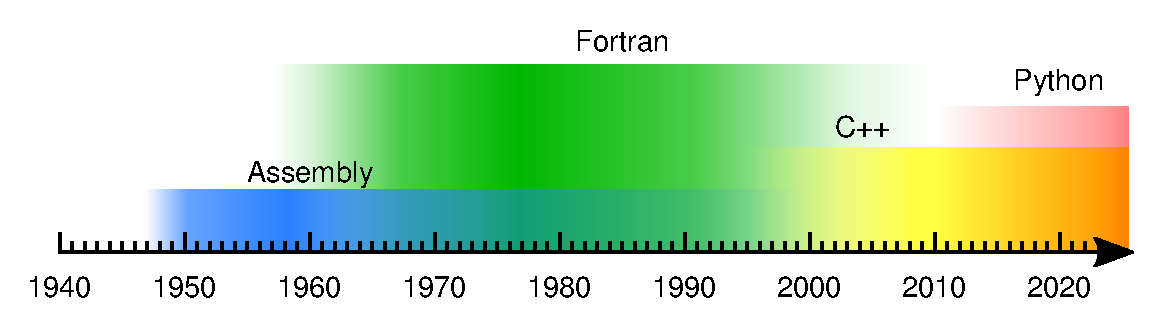
\includegraphics[width=\linewidth]{img/programming-languages.pdf}

\vspace{0.5 cm}
C++ first appeared in 1985: 10--15~years before we adopted it

\vspace{0.25 cm}
Python first appeared in 1990: 20--25~years before we adopted it

\vspace{0.25 cm}
\uncover<2->{Julia first appeared in 2012: maybe we'll be using it by 2030}
\end{frame}

\begin{frame}{An aside on future languages}
\vspace{0.5 cm}
\begin{columns}
\column{0.5\linewidth}
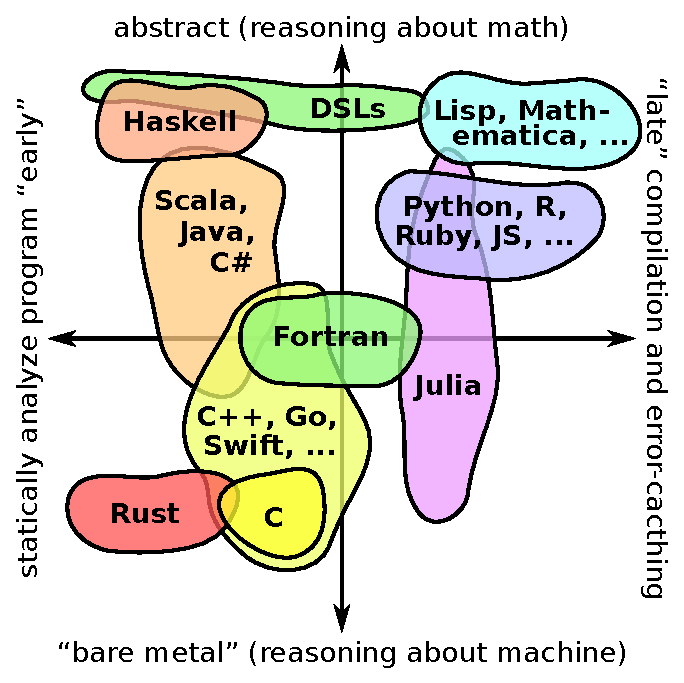
\includegraphics[width=\linewidth]{img/language-properties-grid.pdf}

\column{0.5\linewidth}
\begin{itemize}
\item \textcolor{darkblue}{Python, R, Ruby, Javascript, Lua, etc.} are all relatively abstract, late error-catching glue languages. \\ \uncover<2->{\textcolor{darkblue}{Python isn't special:} it's just where the best libraries self-gravitated.}

\item<3-> \textcolor{darkblue}{Julia} is different: everything just-in-time compiles, so it is just as dynamic, but it can be fast, too.

\item<4-> \textcolor{darkblue}{Rust} is a unique extreme. Triggers?

\item<5-> \textcolor{darkblue}{DSLs (domain specific languages)} have physics concepts baked in with opportunities for strict error checking and flexible backends.

\end{itemize}
\end{columns}
\end{frame}

\begin{frame}{Some DSLs\ldots\ (see Sezen Sekmen @ LHCP 2020)}
\vspace{0.25 cm}
\begin{center}
\begin{onlyenv}<1>
\vspace{-0.25 cm}
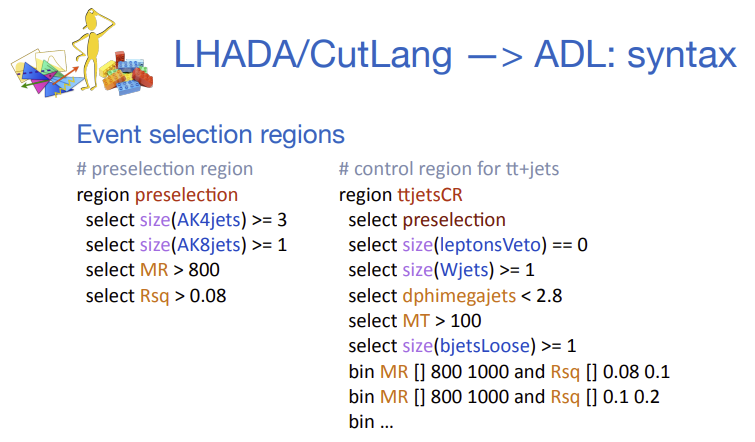
\includegraphics[width=0.8\linewidth]{img/adl-1.png}
\end{onlyenv}
\begin{onlyenv}<2>
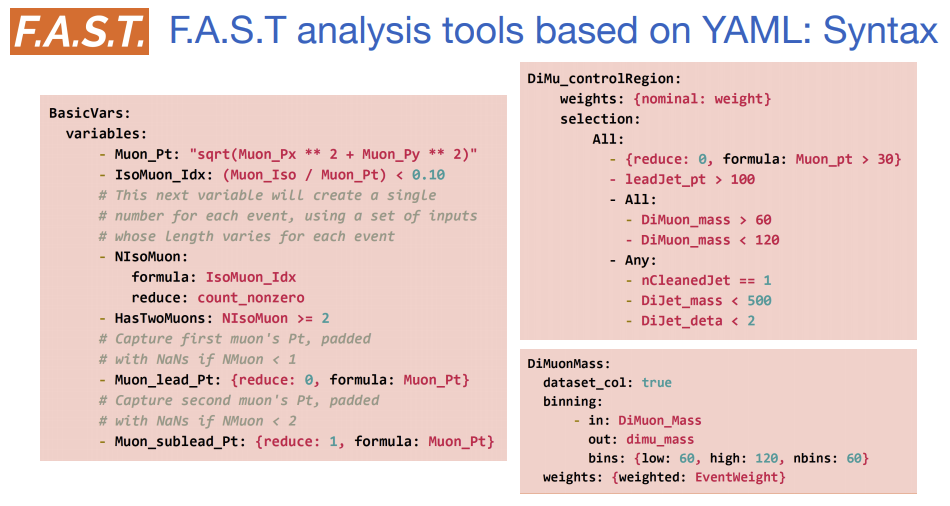
\includegraphics[width=0.9\linewidth]{img/adl-2.png}
\end{onlyenv}
\begin{onlyenv}<3>
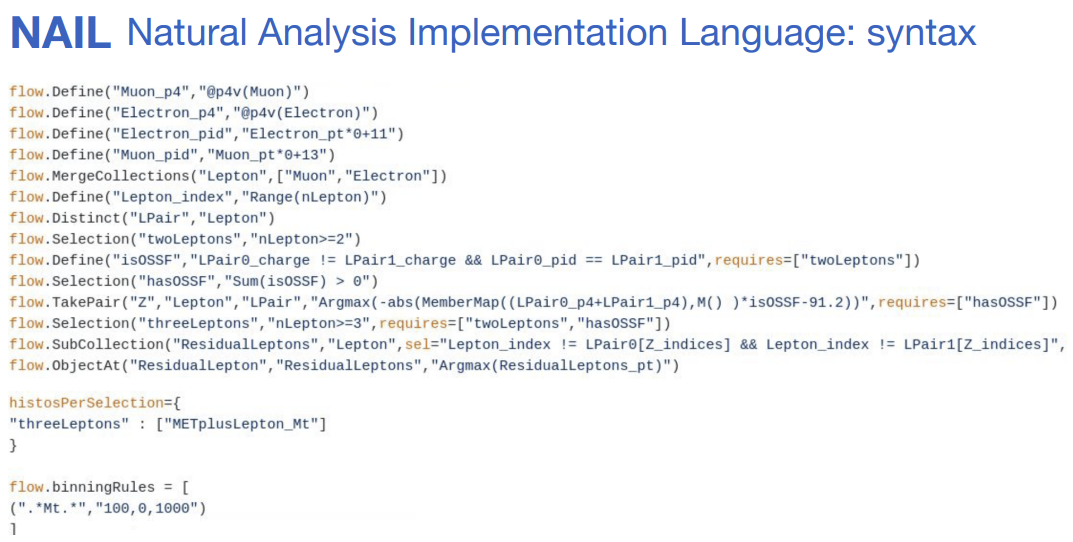
\includegraphics[width=1.0\linewidth]{img/adl-3.png}
\end{onlyenv}
\begin{onlyenv}<4>
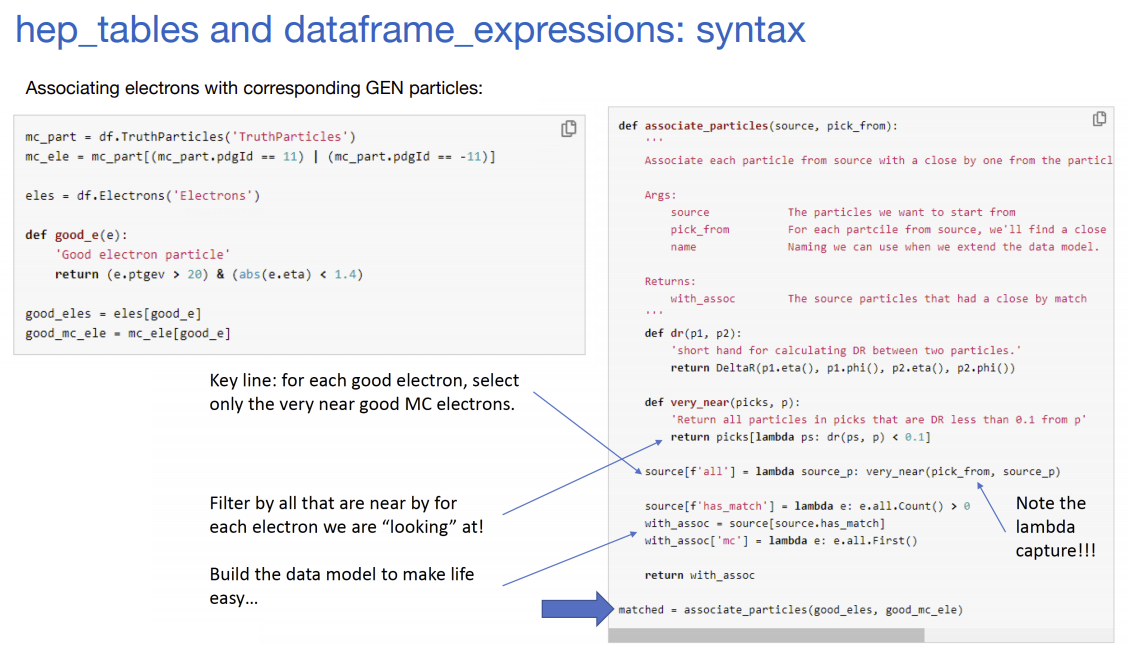
\includegraphics[width=0.9\linewidth]{img/adl-4.png}
\end{onlyenv}
\begin{onlyenv}<5>
PartiQL (demo) $\to$ AwkwardQL (real implementation)\hspace{3.6 cm}

\vspace{0.25 cm}
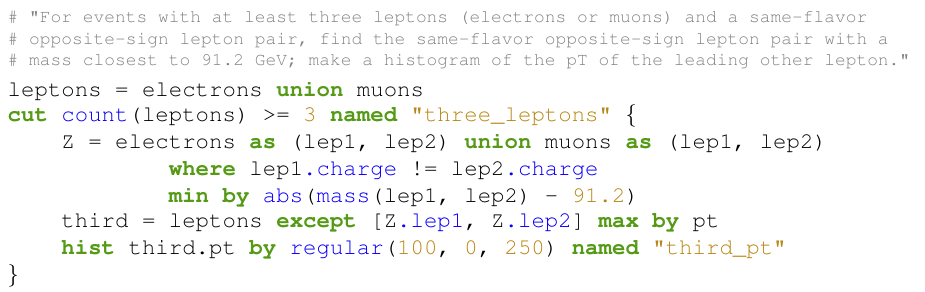
\includegraphics[width=0.9\linewidth]{img/adl-5.png}
\end{onlyenv}
\end{center}
\end{frame}

\begin{frame}{\mbox{ }}
\vspace{0.5 cm}

\begin{center}
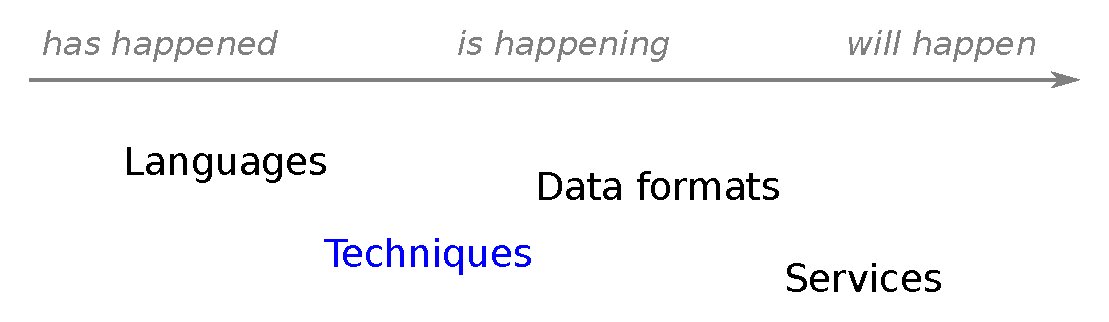
\includegraphics[width=0.9\linewidth]{img/topics-2.pdf}
\end{center}
\end{frame}

\begin{frame}{\mbox{ }}
\vspace{0.5 cm}

\begin{center}
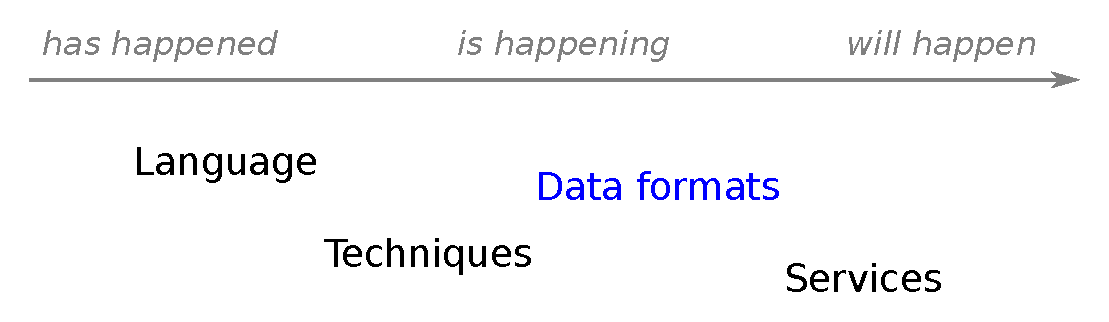
\includegraphics[width=0.9\linewidth]{img/topics-3.pdf}
\end{center}
\end{frame}

\begin{frame}{\mbox{ }}
\vspace{0.5 cm}

\begin{center}
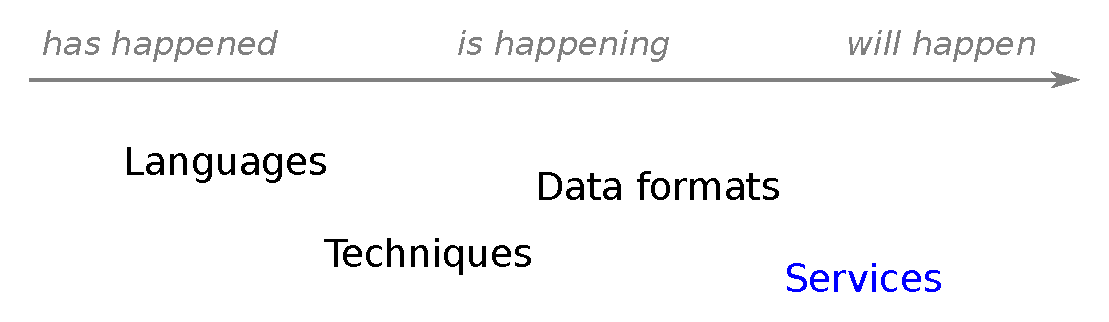
\includegraphics[width=0.9\linewidth]{img/topics-4.pdf}
\end{center}
\end{frame}


\end{document}
